\documentclass[12pt,b5paper]{ltjsarticle}

\usepackage{amssymb}
\pagestyle{empty}

\usepackage{amsmath}	% required for `\align' (yatex added)
\usepackage{graphicx}	% required for `\includegraphics' (yatex added)
\begin{document}

$\displaystyle \frac{0}{0}$
と
$\displaystyle \frac{1}{0}$
について

\quad

割り算は掛け算から出来ている。
次の式のように$\times b$を右辺から消して$\div b$を付け加えている。
\begin{align}
 a \times b = & c \phantom{\div b}\\
 a \hspace*{20pt} = & c \div b
\end{align}

$b=0$であれば$c=0$であるので次のようになる。
\begin{align}
 x \times 0 = & 0 \phantom{\div b}\\
 x \hspace*{20pt} = & 0 \div 0
\end{align}
この場合、$x$はどんな値でもいいので、
$0\div0$は値が一つに定まらない(不定)となる。

$1\div0$は同じように考えると次の式になる
\begin{align}
 x \times 0 = & 1 \phantom{\div b}\\
 x \hspace*{20pt} = & 1 \div 0
\end{align}
$x\times0$は$1$になることはないので
$1\div0$は値を持たない(不能)となる。

$0\div0$は様々な値になり得るが、
$1\div0$はどんな値にもなり得ない。
この為、
$0$で割るのは問題があるが
分けて考える必要がある。



\hrulefill

\begin{equation}
 f(x)=\frac{x+a}{x^2-4}
\end{equation}

$f(x)$は次の場合に分けられる。
\begin{itemize}
 \item 分母が$0$でない場合($x^2-4\ne0$)
 \item 分母と分子がともに$0$の場合($x^2-4=0, x+a=0$)
 \item 分母が$0$で分子$x+a$が$0$でない場合($x^2-4=0, x+a\ne0$)
\end{itemize}

分子が$0$でなく分母が$0$の場合は値がない為、
グラフは上下に伸びた形になる。
分子分母がともに$0$の場合は値が無いわけではなく
定まらないだけで、
グラフは特定の値を取るように考えられる。

$a=2$の時、$f(-2)=1/4$、$a=-2$の時、$f(2)=1/4$



\begin{tabular}{c|c}
 \begin{minipage}{200pt}
  $a=-1$\\
  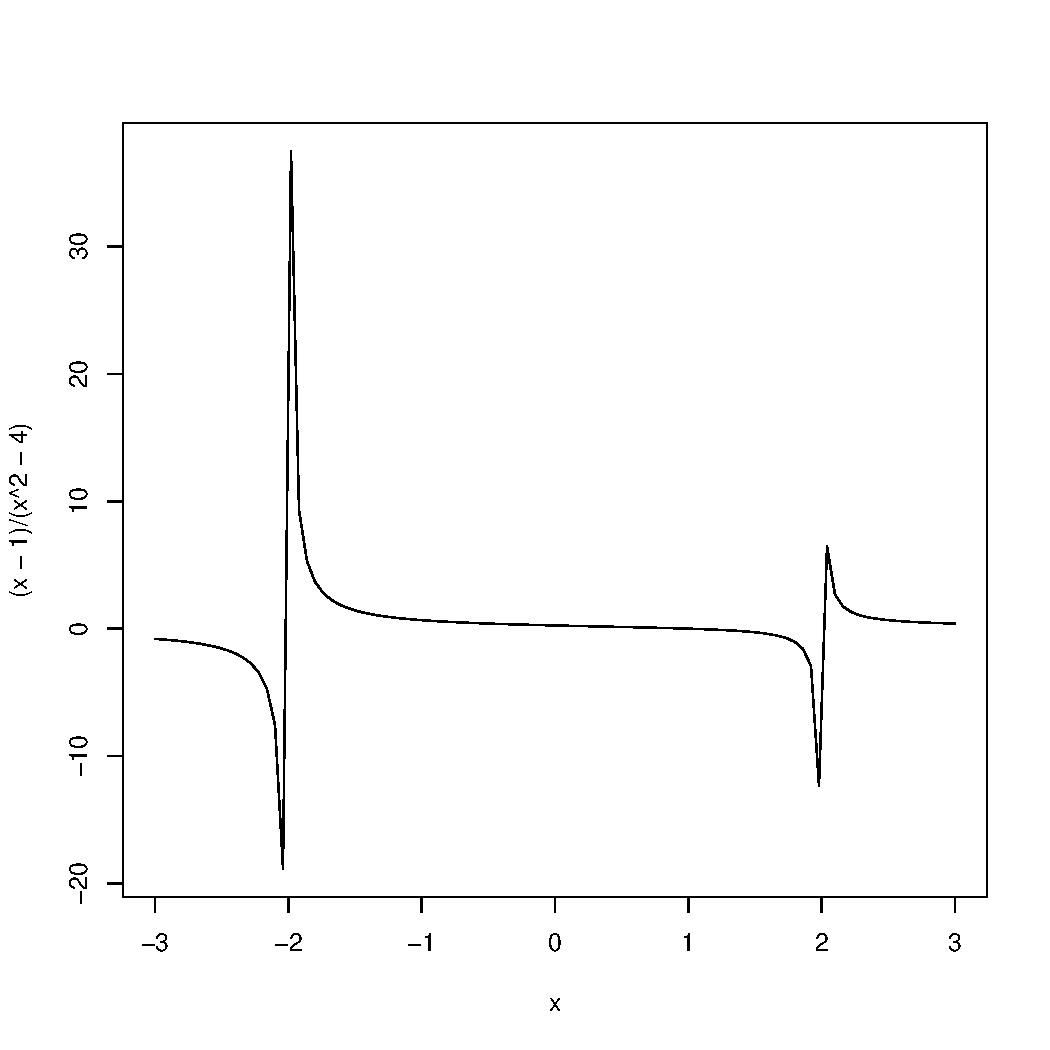
\includegraphics[scale=.35]{m1.pdf}
 \end{minipage} &
 \begin{minipage}{200pt}
  $a=1$\\
  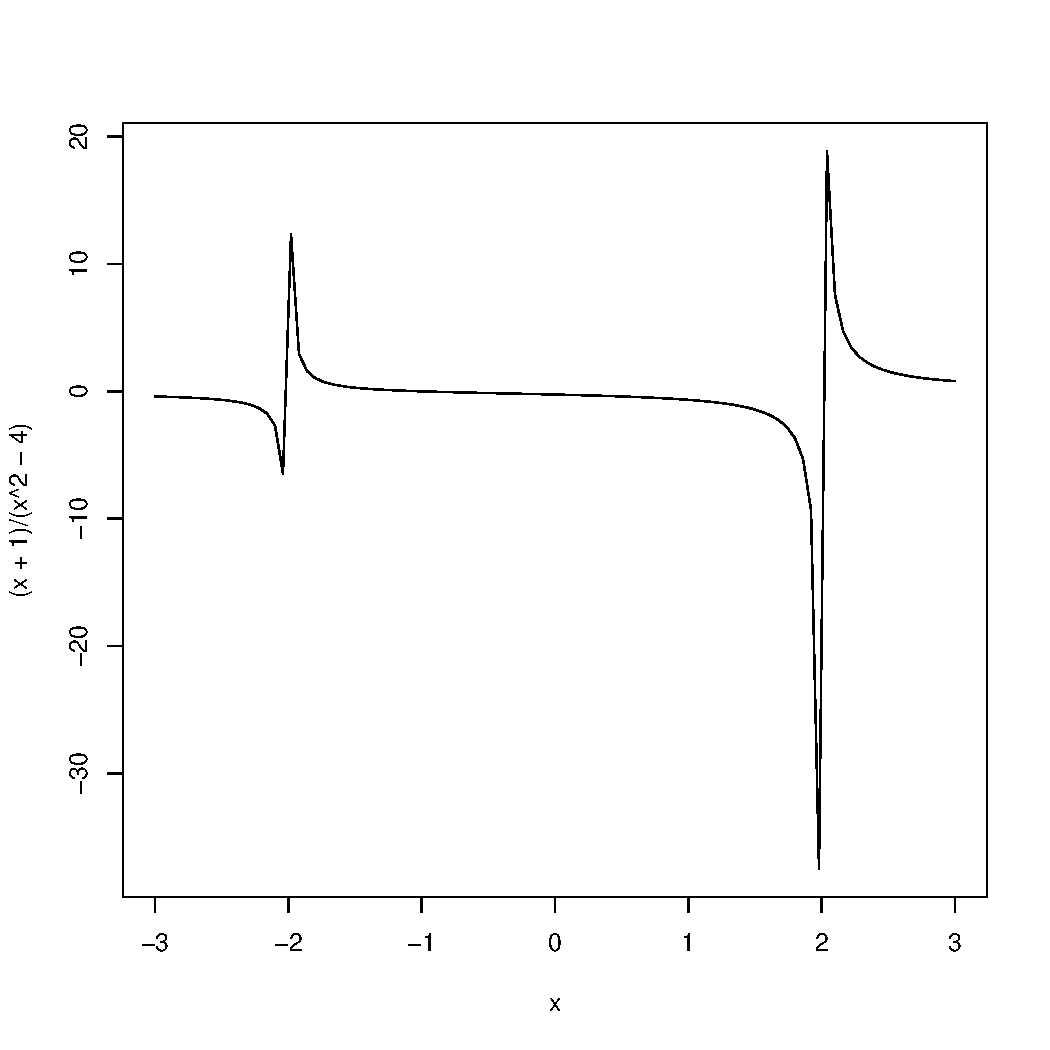
\includegraphics[scale=.35]{p1.pdf}
 \end{minipage}\\ \hline
 \begin{minipage}{200pt}
  $a=-2$\\
  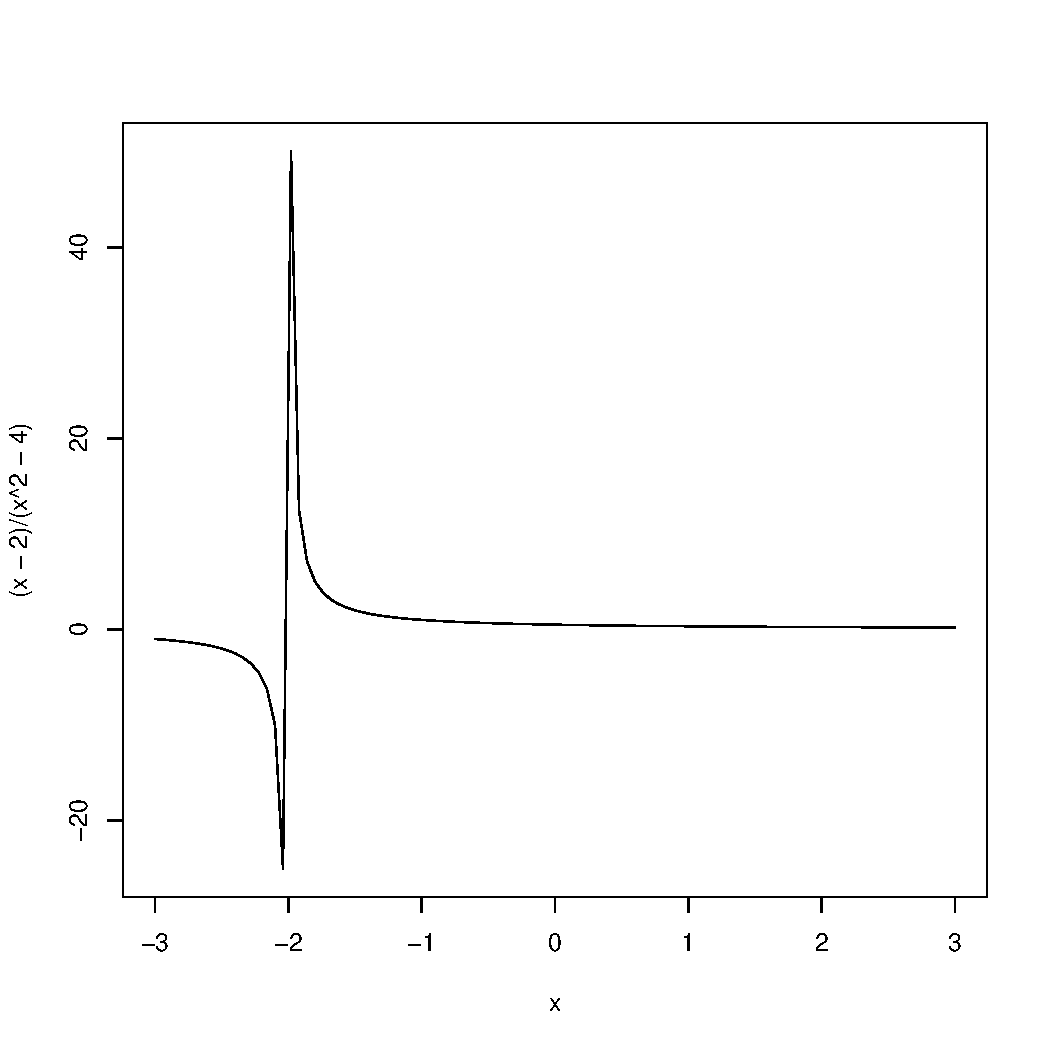
\includegraphics[scale=.35]{m2.pdf}
 \end{minipage} &
 \begin{minipage}{200pt}
  $a=2$\\
  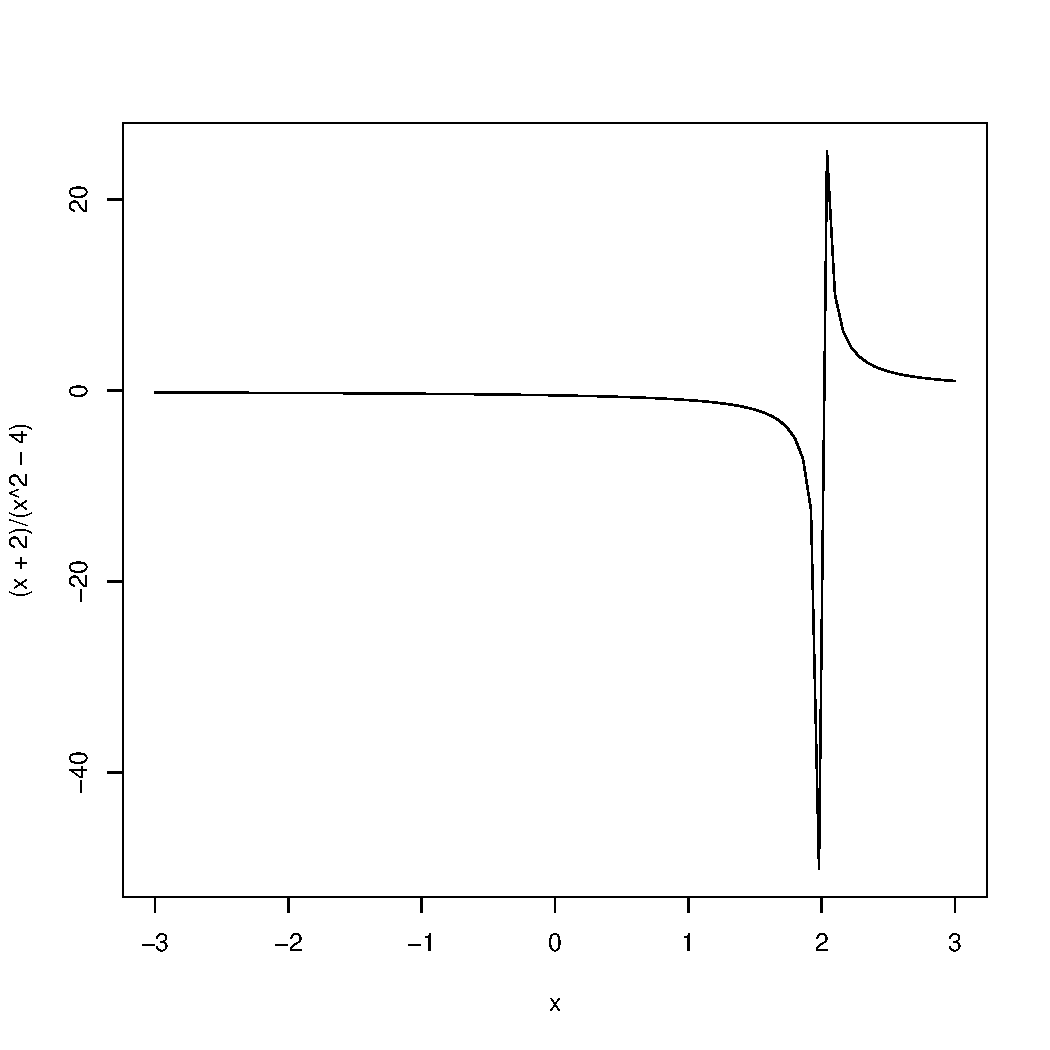
\includegraphics[scale=.35]{p2.pdf}
 \end{minipage}\\ \hline
 \begin{minipage}{200pt}
  $a=-3$\\
  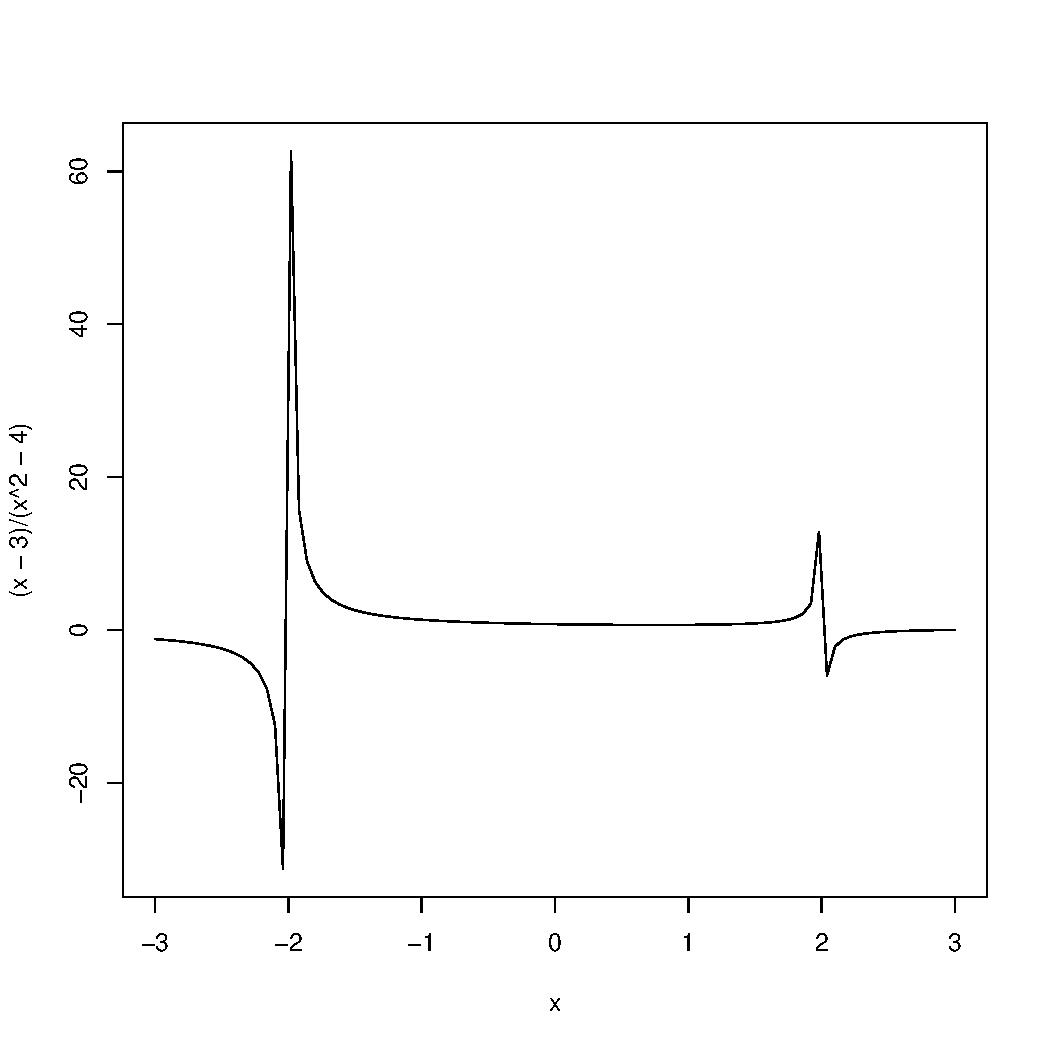
\includegraphics[scale=.35]{m3.pdf}
 \end{minipage} &
 \begin{minipage}{200pt}
  $a=3$\\
  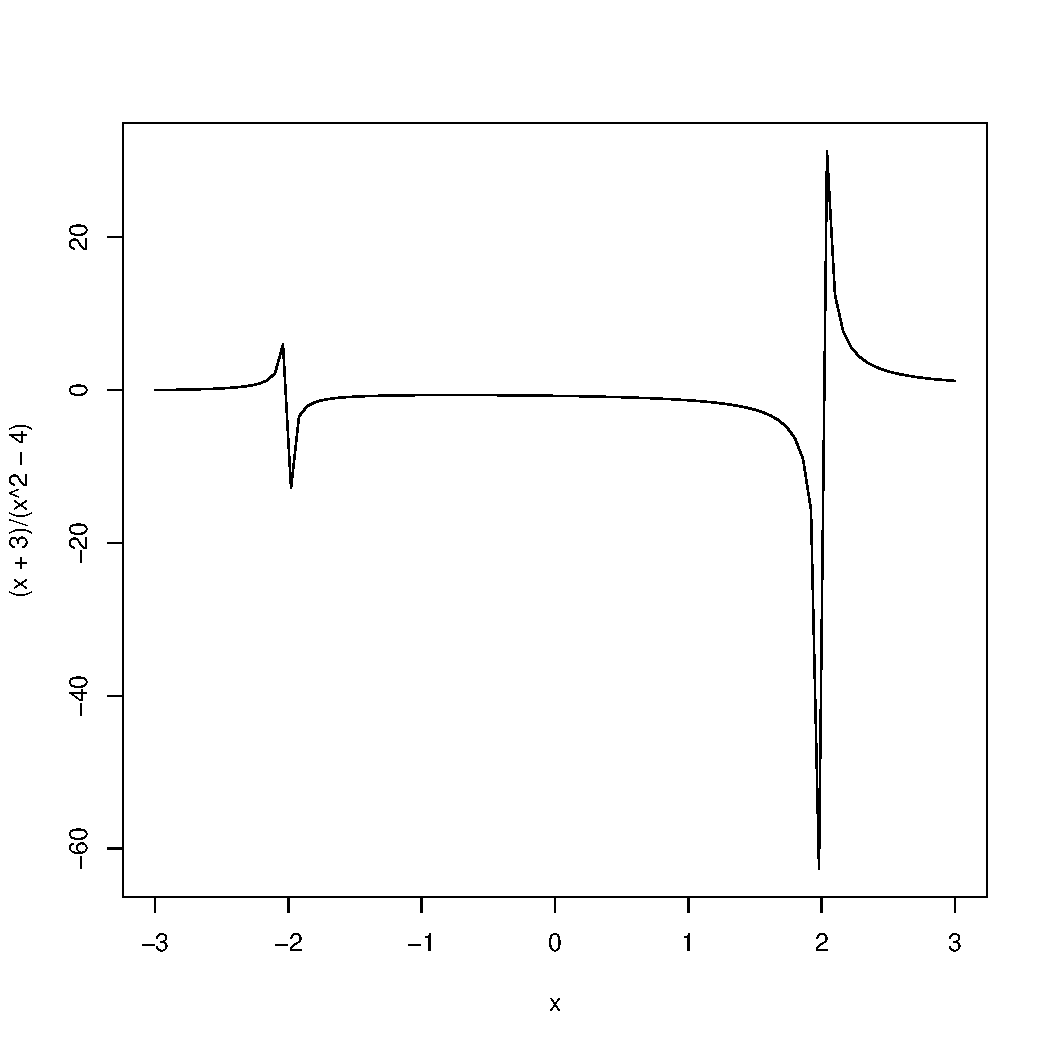
\includegraphics[scale=.35]{p3.pdf}
 \end{minipage}\\
\end{tabular}




\end{document}
